\documentclass[conference]{IEEEtran}
\IEEEoverridecommandlockouts
\usepackage[T1]{fontenc}
\usepackage{amsmath,amssymb}
\usepackage{mathptmx}
\usepackage{microtype}
\usepackage{graphicx}
\usepackage{booktabs}
\usepackage{xurl}
\usepackage[hidelinks]{hyperref}
\graphicspath{{figv/}}
\setlength{\textfloatsep}{10pt plus 2pt minus 2pt}
\setlength{\dbltextfloatsep}{10pt plus 2pt minus 2pt}
\renewcommand{\topfraction}{0.9}
\renewcommand{\dbltopfraction}{0.9}
\renewcommand{\textfraction}{0.08}
\renewcommand{\floatpagefraction}{0.85}
\renewcommand{\dblfloatpagefraction}{0.85}
\setcounter{topnumber}{3}
\setcounter{dbltopnumber}{2}
\DeclareMathOperator{\sign}{sign}
\newcommand{\vect}[1]{\mathbf{#1}}

\begin{document}

\title{ECSE 551 Assignment 1: Lasso and ElasticNet Regression, SVM and MLP Classifiers, and S\&P\,500 Return Prediction}

\author{\IEEEauthorblockN{William Charron-Boyle, Radman Jamalshirpanjeh, Brandon Ku, Jack McDonald}
\IEEEauthorblockA{Department of Electrical and Computer Engineering, McGill University, Montr\'eal, QC, Canada}}

\maketitle

\begin{abstract}
In this assignment we explored two benchmark datasets, built four models from scratch and applied simple models to stock return prediction. Using only NumPy and gradient descent, we implemented Lasso regression with soft thresholding, ElasticNet regression, a one-vs-rest multiclass SVM and a one-hidden-layer MLP. We compared them with scikit-learn's \texttt{LinearRegression} and \texttt{RandomForestClassifier}. On the Diabetes dataset, our Lasso achieved the lowest test MSE (2797, versus 2822 for least squares). On the Digits dataset, the MLP was the most accurate classifier (98.0\%), ahead of the random forest (97.2\%) and the SVM (96.7\%). We then predicted next-day volatility-adjusted S\&P\,500 returns with Lasso, random forest and MLP regressors, retrained every year on a rolling window. All models gave a positive Sharpe ratio on the 2011--2013 test period, ranging from 1.7 to 4.0. Adding sentiment data improved the results only slightly.
\end{abstract}

\section{Introduction}
This assignment has three tasks. Task~1 explores two scikit-learn datasets. The Diabetes dataset~\cite{skDiab} contains 442 patients and ten baseline variables: age, sex, body mass index (\texttt{bmi}), blood pressure (\texttt{bp}) and six serum measurements (\texttt{s1}--\texttt{s6}). Its target is a continuous measure of disease progression after one year. The Digits dataset~\cite{skDig} contains 1797 handwritten digits stored as $8\times8$ images, giving 64 pixel features with a label from 0 to 9.

Task~2 asks us to implement two regression models (ElasticNet and Lasso) and two classifiers (a multiclass SVM and an MLP) using only NumPy~\cite{numpy} and gradient descent. We compare them with \texttt{LinearRegression}~\cite{skLinReg} and \texttt{RandomForestClassifier}~\cite{skRF}. Every model uses a 70/30 train/test split with random state 42, and hyperparameters are chosen by 5-fold cross-validation (CV) on the training set.

Task~3 uses daily returns of S\&P\,500 stocks from 1980 to 2013, plus sentiment data for 2009--2015. The goal is to predict each stock's volatility-adjusted return for tomorrow, using only information available today, which we do with Lasso, random forest and MLP regressors from scikit-learn. We evaluate predictions with the Sharpe ratio, the profit-and-loss (PnL) curve, the cumulative rank correlation and the average holding period.

In short, regularisation helps only a little on Diabetes, but it makes the coefficients easier to interpret. On Digits, the non-linear models beat the linear SVM by a small margin. On the stock data, simple reversal and low-volatility signals give a weak but consistent edge out of sample. However, the best models change their positions almost every day.

\section{Datasets}
\subsection{Diabetes and Digits}
Neither dataset needed cleaning: there are no missing, infinite or duplicated values, and every value lies in a valid range. The Diabetes target ranges from 25 to 346, and the Digits pixels are integers from 0 to 16. Scikit-learn already centres and scales the Diabetes features (every feature has mean 0 and standard deviation $\approx0.048$), while the raw units vary widely, for example 19--79 for age. We still standardised both datasets using statistics from the training split only.

Fig.~\ref{fig:diab_hist} shows that all Diabetes features are unimodal except \texttt{sex}, which is binary. The features \texttt{bmi}, \texttt{s3} and \texttt{s4} are right-skewed, \texttt{s4} is nearly discrete, and none has heavy tails. Box plots (in the notebook) show only a few outliers, and they are plausible values, so we kept them. Scatter plots of each feature against the target show roughly linear but noisy relationships, and \texttt{s1} against \texttt{s2} is almost a straight line. In the correlation matrix (Fig.~\ref{fig:diab_corr}), \texttt{bmi} ($r=0.59$) and \texttt{s5} ($r=0.57$) are the features most correlated with the target. Two pairs of features are strongly correlated with each other: \texttt{s1}--\texttt{s2} ($r=0.90$) and \texttt{s3}--\texttt{s4} ($r=-0.74$). This collinearity is a good reason to try regularisation.

\begin{figure*}[t]
\centering
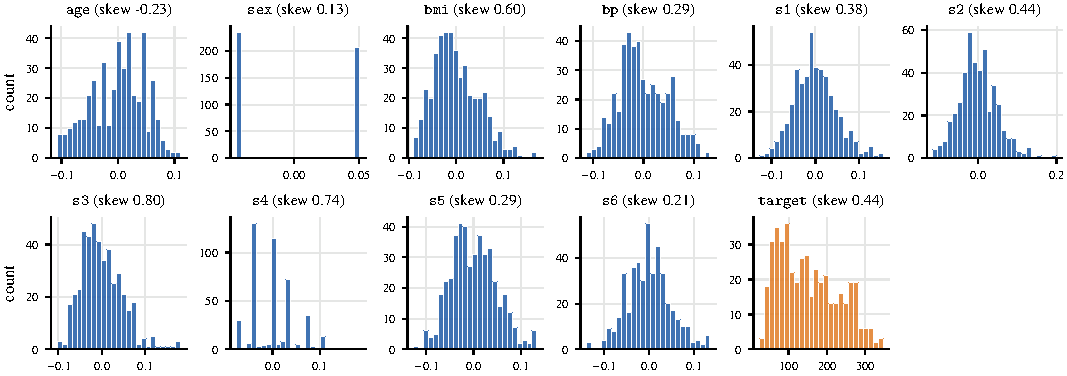
\includegraphics[width=\textwidth]{diab_hist.pdf}
\caption{Distributions of the Diabetes features and target. \texttt{sex} is binary, \texttt{s4} is nearly discrete, and the other features are unimodal and mostly slightly right-skewed.}
\label{fig:diab_hist}
\end{figure*}

\begin{figure}[t]
\centering
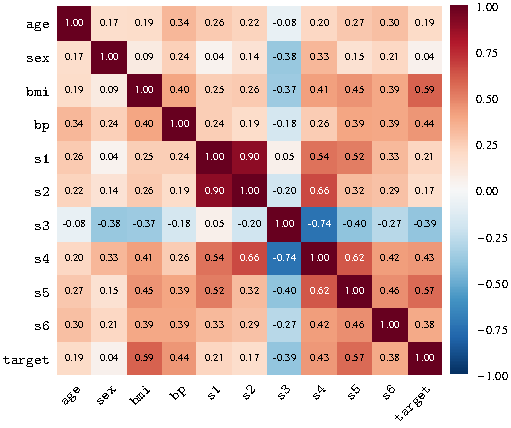
\includegraphics[width=\columnwidth]{diab_corr.pdf}
\caption{Pearson correlation matrix of the Diabetes data. Note the strongly correlated pairs \texttt{s1}--\texttt{s2} and \texttt{s3}--\texttt{s4}.}
\label{fig:diab_corr}
\end{figure}

The ten Digits classes are balanced (174--183 images each), so accuracy is a fair metric. Almost half of all pixel values are zero. Pixels on the edges of the image are nearly always zero, while central pixels tend to be either very dark or very light (Fig.~\ref{fig:dig_stats}). Since the pixel variances differ a lot, we standardised the pixels. Most pixel pairs are only weakly correlated: 90.5\% of the pairs have $|r|<0.3$.

\begin{figure}[t]
\centering
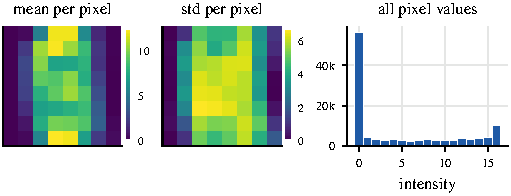
\includegraphics[width=\columnwidth]{digits_stats.pdf}
\caption{Digits: mean and standard deviation of each pixel, and the histogram of all pixel values.}
\label{fig:dig_stats}
\end{figure}

\subsection{S\&P\,500 returns and sentiment}
The return file covers 8577 trading days and 1335 stocks. The membership file marks between 489 and 500 index members on each day, and no member has a missing return. We only make and evaluate predictions for stocks that are members on day $t$. The Psychsignal sentiment data start in July 2009, but they cover few members: on average, 57 members per day in 2009, rising to 233 in 2013.

\section{Methodology}
The equations in this section follow the course lecture notes~\cite{notes}. All from-scratch models are trained with gradient descent, $\theta_{t+1}=\theta_t-\eta\,\vect{g}_t$, where $\vect{g}_t$ is the gradient (or subgradient) of the loss and $\eta$ is the learning rate. Hyperparameters are chosen by 5-fold CV, which estimates the risk of a setting $\lambda$ as $R^{\mathrm{cv}}_\lambda=\frac{1}{K}\sum_{k=1}^{K}R_0\big(\hat\theta_\lambda(\mathcal{D}_{-k}),\mathcal{D}_k\big)$ with $K=5$~\cite{notes}. In words, each model is trained on four folds and tested on the remaining one, and the five scores are averaged. We used the same folds (\texttt{KFold}~\cite{skKFold}) for every model.

\subsection{Regression models}
Let $\vect{X}$ be the $m\times n$ standardised feature matrix, $\vect{y}$ the targets, $\vect{w}$ the weights and $b$ the bias, which is never penalised. We report the mean squared error, $\mathrm{MSE}=\frac{1}{m}\sum_i(y_i-\hat y_i)^2$, and the coefficient of determination, $R^2=1-\sum_i(y_i-\hat y_i)^2/\sum_i(y_i-\bar y)^2$, which is the fraction of the target variance explained by the model.

\textit{Linear regression.} \texttt{LinearRegression} computes the ordinary least squares (OLS) solution $\hat{\vect{w}}=(\vect{X}^\top\vect{X})^{-1}\vect{X}^\top\vect{y}$~\cite{notes}, with no penalty. It serves as our baseline.

\textit{Lasso.} Lasso adds an $\ell_1$ penalty to the squared error, which pushes some weights to exactly zero:
\begin{equation}
\min_{\vect{w},b}\ \frac{1}{2m}\|\vect{y}-(\vect{X}\vect{w}+b\vect{1})\|_2^2+\lambda\|\vect{w}\|_1 .
\label{eq:lasso}
\end{equation}
Since $|w_j|$ has no derivative at zero, we used the proximal gradient method from Lecture~8. Each iteration first takes a normal gradient step on the squared error,
\begin{equation}
\vect{v}=\vect{w}+\frac{\eta}{m}\vect{X}^\top\big(\vect{y}-\vect{X}\vect{w}-b\vect{1}\big),
\end{equation}
and then applies soft thresholding to each weight:
\begin{equation}
w_j\leftarrow S_{\eta\lambda}(v_j)=\sign(v_j)\max\big(|v_j|-\eta\lambda,\,0\big).
\label{eq:soft}
\end{equation}
Weights smaller than $\eta\lambda$ in magnitude become exactly zero, and all other weights move towards zero by $\eta\lambda$.

\textit{ElasticNet.} ElasticNet uses both an $\ell_1$ and an $\ell_2$ penalty:
\begin{equation}
\min_{\vect{w},b}\ \frac{1}{2m}\|\vect{y}-(\vect{X}\vect{w}+b\vect{1})\|_2^2+\lambda_1\|\vect{w}\|_1+\frac{\lambda_2}{2}\|\vect{w}\|_2^2 .
\label{eq:enet}
\end{equation}
The $\ell_2$ term encourages correlated features to share similar weights, whereas Lasso tends to keep only one of them~\cite{notes}. We used a single penalty, $\lambda=\lambda_1=\lambda_2$, and plain subgradient descent with $\sign(w_j)$ as the subgradient of $|w_j|$:
\begin{equation}
\vect{w}\leftarrow\vect{w}-\eta\Big(-\tfrac{1}{m}\vect{X}^\top\vect{r}+\lambda\,\sign(\vect{w})+\lambda\vect{w}\Big),
\end{equation}
where $\vect{r}=\vect{y}-\vect{X}\vect{w}-b\vect{1}$ is the residual.

\textit{Learning rate and tuning.} Gradient descent becomes unstable if $\eta$ is too large compared with the largest eigenvalue $L$ of $\vect{X}^\top\vect{X}/m$ (plus $\lambda$ for ElasticNet). On our training data $L=3.96$, so we used $\eta=0.25$ for Lasso and $\eta=\min(0.25,\,1/(3.96+\lambda))$ for ElasticNet, with 5000 iterations each. We then chose $\lambda$ from 25 values between $10^{-2}$ and $10^{2}$ using the CV MSE.

\subsection{Classification models}
\textit{Multiclass SVM.} A binary SVM uses the decision function $f(\vect{x})=\vect{w}^\top\vect{x}+w_0$ with labels $\tilde y_i\in\{-1,+1\}$. As shown in Lecture~8, the soft-margin SVM is equivalent to minimising the hinge loss with an $\ell_2$ penalty:
\begin{equation}
\min_{\vect{w},w_0}\ \frac12\|\vect{w}\|_2^2+\gamma\sum_{i=1}^{m}\max\big(0,\,1-\tilde y_i(\vect{w}^\top\vect{x}_i+w_0)\big).
\label{eq:hinge}
\end{equation}
Following the class template, we wrote the penalty as $\lambda\|\vect{w}\|^2$ and averaged the hinge losses over the samples. This is the same problem, rescaled, with $\gamma=1/(2\lambda m)$. Only the samples inside the margin, $S=\{i:\tilde y_i f(\vect{x}_i)<1\}$, contribute to the subgradient, which gives the updates
\begin{equation}
\vect{w}\leftarrow\vect{w}-\eta\Big(2\lambda\vect{w}-\frac1m\sum_{i\in S}\tilde y_i\vect{x}_i\Big),\quad w_0\leftarrow w_0+\frac{\eta}{m}\sum_{i\in S}\tilde y_i .
\end{equation}
For ten classes, we trained one classifier per digit (that digit against all the others) and predicted the digit with the highest score~\cite{notes}. We searched $\eta$ from 0.001 to 3 and $\lambda$ from $10^{-4}$ to 1, and then tuned the number of iterations.

\textit{MLP.} Each layer of an MLP computes $\vect{z}_\ell=\varphi(\vect{b}_\ell+\vect{W}_\ell\vect{z}_{\ell-1})$~\cite{notes}. Our network has one hidden layer of $H$ units with the activation $\mathrm{ReLU}(a)=\max(a,0)$, followed by a softmax output, $\mu_c=e^{a_c}/\sum_{c'}e^{a_{c'}}$, which gives one probability per digit. We trained it with full-batch gradient descent on the cross-entropy loss from Lecture~6:
\begin{equation}
\mathrm{NLL}(\theta)=-\frac{1}{m}\sum_{i=1}^{m}\sum_{c=1}^{10}y_{ic}\log\mu_{ic},
\label{eq:ce}
\end{equation}
where $y_{ic}$ is the one-hot label (from \texttt{OneHotEncoder}~\cite{skPre}). The gradients are computed by backpropagation, i.e.\ the chain rule applied layer by layer. At the output, the gradient is simply $(\boldsymbol{\mu}-\vect{y})/m$, and it is passed back through the ReLU, whose derivative is 1 for positive inputs and 0 otherwise. We searched $H$ from 8 to 512 and $\eta$ from 0.01 to 2, and then tuned the number of epochs.

\textit{Random forest.} A random forest averages many decision trees. Each tree is trained on a bootstrap sample of the data and considers a random subset of features at each split, which reduces variance~\cite{skRF}. We tuned the number of trees ($\{50,100,300\}$), the maximum depth ($\{\text{none},10,20\}$), the number of features per split ($\sqrt{n}$ or $\log_2 n$) and the minimum leaf size ($\{1,2\}$) with \texttt{GridSearchCV}~\cite{skGS}, using the same five folds. The classifiers are compared using accuracy, i.e.\ the fraction of test images whose predicted digit matches the true label, and using confusion matrices, which show which digits get mixed up.

\subsection{Return prediction}
\textit{Problem formulation.} We treat Task~3 as a cross-sectional regression problem. On each trading day $t$, for every stock that is an S\&P\,500 member on that day (about 500 stocks, well above the required 100), we predict the stock's volatility-adjusted return for day $t+1$ using only information available at the close of day $t$. Only the relative ordering of the stocks matters for a market-neutral portfolio, so the target is demeaned across stocks every day. We use the return data from 1981 to 2010 for training, with 2001--2010 serving as a validation period for choosing hyperparameters, and we keep 2011--2013 as the test set, as required by the assignment. The models are judged with the Sharpe ratio of the resulting portfolio, its PnL curve, the cumulative rank correlation and the average holding period.

\textit{Volatility adjustment.} As described in the assignment, we track each stock's mean and variance with two exponentially weighted moving averages (EWMA): $\hat\mu_t=(1-\beta_2)r_t+\beta_2\hat\mu_{t-1}$ and $\hat\sigma_t^2=(1-\beta_1)(r_t-\hat\mu_t)^2+\beta_1\hat\sigma_{t-1}^2$, with $\beta_1=0.97$ and $\beta_2=0.99$. We drop the first 60 days of each stock as a burn-in period, while the estimates settle. The adjusted return is $\tilde r_t=r_t/\hat\sigma_{t-1}$.

\textit{Exploratory analysis.} Volatility adjustment brings the standard deviation of member returns from 0.024 to about 1.06, and the adjusted series look roughly stationary. We built six candidate features on day $t$: the last return (\texttt{rev1}), the average return over 5, 20 and 60 days (\texttt{rev5}, \texttt{mom20}, \texttt{mom60}), a longer-term average that skips the most recent month (\texttt{mom250}), and the log volatility (\texttt{vol}). Before modelling, we measured each feature's average daily Spearman correlation with the next-day return (Table~\ref{tab:ic}). Every signal is very weak on its own ($|\rho|\le0.03$), so the data have a very low signal-to-noise ratio. The signs show short-term reversal (recent winners tend to fall back), long-term momentum and a preference for low-volatility stocks. The one-day reversal \texttt{rev1} was close to zero before 2000 but clearly negative afterwards, which shows that these relationships change over time.

\begin{table}[t]
\centering
\caption{Average daily rank correlation of each feature with the next-day return}
\label{tab:ic}
\footnotesize\setlength{\tabcolsep}{3.5pt}
\begin{tabular}{lcccccc}
\toprule
 & rev1 & rev5 & mom20 & mom60 & mom250 & vol\\
\midrule
1981--2000 & 0.001 & $-0.029$ & $-0.018$ & $-0.011$ & 0.012 & $-0.016$\\
2001--2010 & $-0.021$ & $-0.014$ & $-0.009$ & $-0.005$ & 0.011 & $-0.011$\\
\bottomrule
\end{tabular}
\end{table}

\textit{Data processing and leakage control.} The adjusted returns are clipped to $\pm5$ so that a few extreme days do not dominate training. On each day, every feature is standardised across the member stocks (a cross-sectional z-score) and clipped to $\pm3$. We prevented look-ahead in four ways: (i) $\tilde r_t$ uses the volatility from day $t-1$; (ii) every feature on day $t$ uses only returns up to day $t$; (iii) a model used in year $Y$ is trained only on data from before year $Y$, and we drop the last training day so that no training target overlaps the prediction period; and (iv) all hyperparameters are chosen on 2001--2010, so the test years are never used for tuning.

\textit{Models and tuning.} We compared three simple predictors from scikit-learn: \texttt{Lasso}~\cite{skLasso}, which minimises the same objective as~\eqref{eq:lasso}; \texttt{RandomForestRegressor}~\cite{skRF}; and \texttt{MLPRegressor}~\cite{skMLP}. Each model is retrained every January on the previous $W$ years (a rolling window). For Lasso, we searched $W\in\{5,10,20\}$ years and $\alpha\in\{10^{-4},10^{-3},3\cdot10^{-3},10^{-2}\}$. The random forest uses 50 trees, considers half of the features at each split, and was tuned over (maximum depth, minimum leaf size) $\in\{(4,500),(8,200),(12,100)\}$. The MLP uses an $\ell_2$ penalty of $10^{-3}$ and early stopping, and we tried hidden layers of $(8)$, $(32)$ and $(32,16)$. To keep training fast, the random forest and the MLP are trained on 200\,000 randomly sampled rows from each window. Finally, we can smooth each stock's predictions over time with an EWMA of half-life $h\in\{0,1,2,5,10,20\}$ days.

\textit{Design rationale.} Because the signal is weak and noisy, overfitting is the main risk, so every choice favours simple and stable models. Lasso's $\ell_1$ penalty can remove features that do not help, although with the selected small penalty it kept all six. The random forest uses large minimum leaf sizes and limited depth, and the MLP is small, penalised and stopped early. The rolling window lets the models adapt as relationships such as the \texttt{rev1} reversal change over time, while ten years still give enough data to average out the noise. Demeaning the target removes the market's overall direction, so the models must actually separate good stocks from bad ones instead of profiting from the market's positive drift. Finally, smoothing is a cheap way to lengthen holding periods, since fast-changing predictions would be expensive to trade.

\textit{Metrics.} On each day, the predictions $\hat r_{t,i}$ are demeaned across stocks, making the portfolio market neutral in volatility-adjusted terms, and scaled so that $\sum_i|\hat r_{t,i}|=1$. The daily PnL and the annualised Sharpe ratio are
\begin{equation}
R_t=\sum_i\tilde r_{t+1,i}\,\hat r_{t,i},\qquad \mathrm{SR}=\sqrt{252}\,\frac{\mathbb{E}[R_t]}{\sqrt{\mathrm{var}[R_t]}},
\label{eq:sharpe}
\end{equation}
with the benchmark set to zero and 252 trading days per year. We chose the Sharpe ratio because it measures return per unit of risk, which is what matters for a trading strategy and is much easier to interpret than an MSE on noisy returns. The cumulative PnL curve shows whether performance is steady over time or comes from a few good periods. We use the Spearman (rank) correlation because it checks whether the predicted ordering of stocks is right, and it is less sensitive to extreme returns than Pearson correlation. The average holding period,
\begin{equation}
H_{av}=\frac{1}{N}\sum_{i=1}^{N}\frac{\sum_{t}|\hat r_{t,i}|}{\sum_{t}|\hat r_{t,i}-\hat r_{t-1,i}|},
\label{eq:hold}
\end{equation}
where $N$ is the number of stocks, estimates how many days a position is kept, which is a proxy for trading costs. Finally, the correlation of $R_t$ with an equal-weighted long-only portfolio of the members checks how much the strategy simply follows the market.

\section{Results}
\subsection{Regression on Diabetes}
With $\lambda=1$, Lasso stayed stable up to $\eta=0.5$ and ElasticNet up to about $\eta=0.4$, which matches the limits $2/L$ we expected. Fig.~\ref{fig:paths} shows how the weights change as $\lambda$ grows. Lasso sets weights to exactly zero one by one: \texttt{s2} is the first to stay at zero, and \texttt{bmi} is the last, at $\lambda\approx68$. The last three weights to vanish are \texttt{bp}, \texttt{s5} and \texttt{bmi}, the features most correlated with the target. The earlier order does not follow the marginal correlations (\texttt{sex}, the least correlated feature, survives until $\lambda=10$), because Lasso keeps a feature for what it adds given the other features, not for its correlation alone. ElasticNet shrinks the weights more smoothly, but they never reach exactly zero. This is a side effect of the subgradient update: the weights jump back and forth around zero instead of settling on it.

\begin{figure*}[t]
\centering
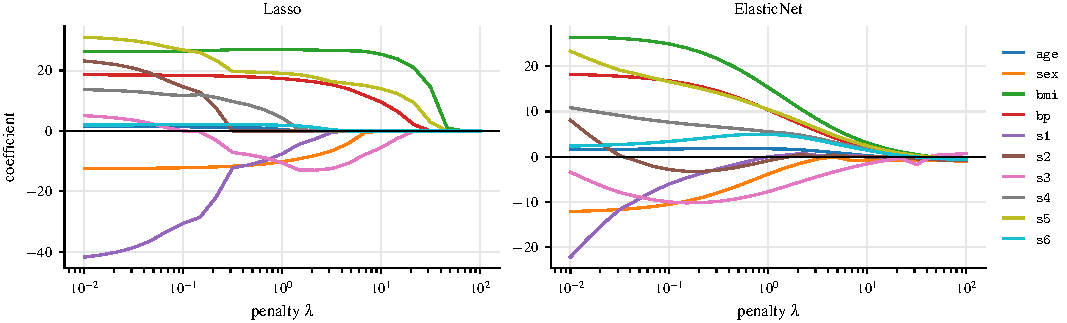
\includegraphics[width=\textwidth]{paths.pdf}
\caption{Coefficient paths for Lasso (left) and ElasticNet (right) as the penalty $\lambda$ increases. Lasso produces exact zeros, while ElasticNet shrinks the weights smoothly.}
\label{fig:paths}
\end{figure*}

Cross-validation selected $\lambda=0.681$ for Lasso and $\lambda=0.068$ for ElasticNet. Both improved the CV MSE by only about 1\% compared with no penalty. Table~\ref{tab:reg} shows that both of our models beat \texttt{LinearRegression} on the test set by a small margin, and all three explain about 48\% of the variance. The gains are small because OLS barely overfits here: its training and test errors are close. The weights differ more than the errors. OLS gives large weights of opposite sign to the correlated pair \texttt{s1} ($-43.3$) and \texttt{s2} ($+24.3$). Lasso removes \texttt{s2} completely and reduces \texttt{s1} to $-9.8$, which makes the model easier to interpret at no cost in accuracy.

\begin{table}[t]
\centering
\small
\caption{Diabetes regression results on the test set}
\label{tab:reg}
\setlength{\tabcolsep}{3.5pt}
\begin{tabular}{lcccc}
\toprule
Model & $\lambda$ & Train MSE & Test MSE & $R^2$\\
\midrule
LinearRegression (sklearn) & -- & 2924.0 & 2821.8 & 0.477\\
Lasso (ours) & 0.681 & 2948.1 & \textbf{2796.6} & \textbf{0.482}\\
ElasticNet (ours) & 0.068 & 2953.6 & 2809.3 & 0.480\\
\bottomrule
\end{tabular}
\end{table}

\subsection{Classification on Digits}
\textit{SVM.} Fig.~\ref{fig:tuning}(a)--(b) shows that the SVM reaches about 94--95.5\% CV accuracy over a wide range of settings. It fails only when both $\eta$ and $\lambda$ are large, because the updates then become unstable. The best setting was $\eta=1$, $\lambda=0.003$ and 500 iterations, which gave 96.7\% test accuracy. The loss converged within about 100 iterations.

Fig.~\ref{fig:svm_scores} shows the decision boundary of each one-vs-rest classifier on the test set. For classifier $c$, the score $f_c(\vect{x})=\vect{w}_c^\top\vect{x}+b_c$ of every test image is plotted, and the boundary $f_c(\vect{x})=0$ is drawn in red. Digits 0, 2, 4, 6 and 7 are almost perfectly separated from the rest, with at most two mistakes each. Digits 1, 3, 8 and 9 overlap the boundary the most, and digits 8 and 9 have 11 misclassified test images each. Many images of these digits fall on the wrong side of their own boundary, but the final multiclass prediction still gets most of them right, because it picks the class with the highest score rather than requiring a positive one.

\begin{figure*}[t]
\centering
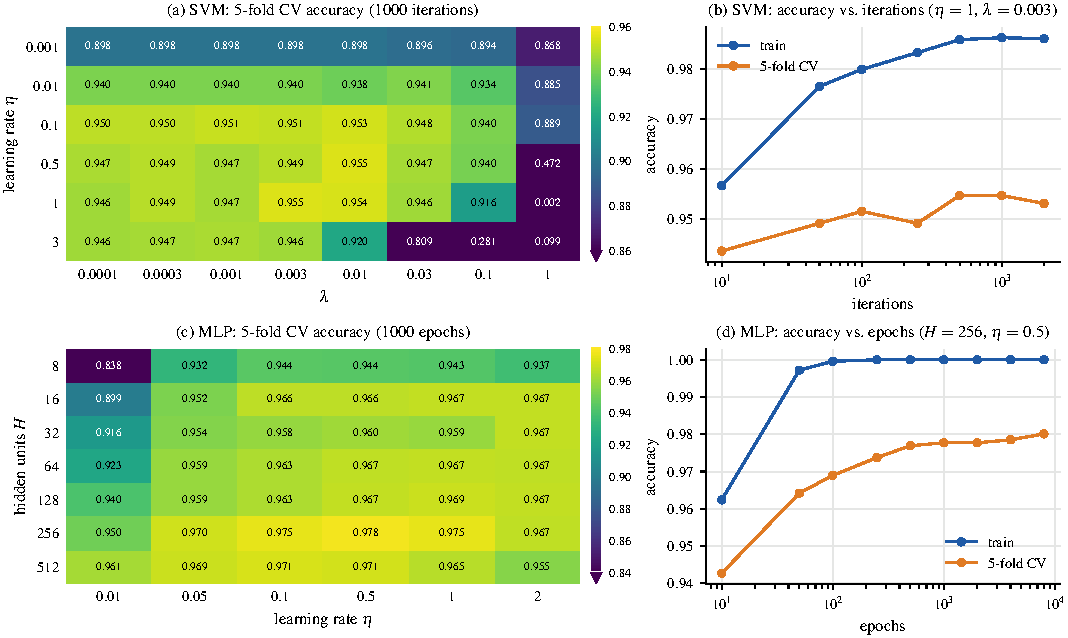
\includegraphics[width=\textwidth]{tuning.pdf}
\caption{Hyperparameter tuning of our classifiers on Digits. (a) SVM 5-fold CV accuracy for each learning rate and $\lambda$; cells below 0.86 are diverged runs. (b) SVM training and CV accuracy against the number of iterations. (c) MLP 5-fold CV accuracy for each hidden size and learning rate. (d) MLP training and CV accuracy against the number of epochs.}
\label{fig:tuning}
\end{figure*}

\begin{figure*}[t]
\centering
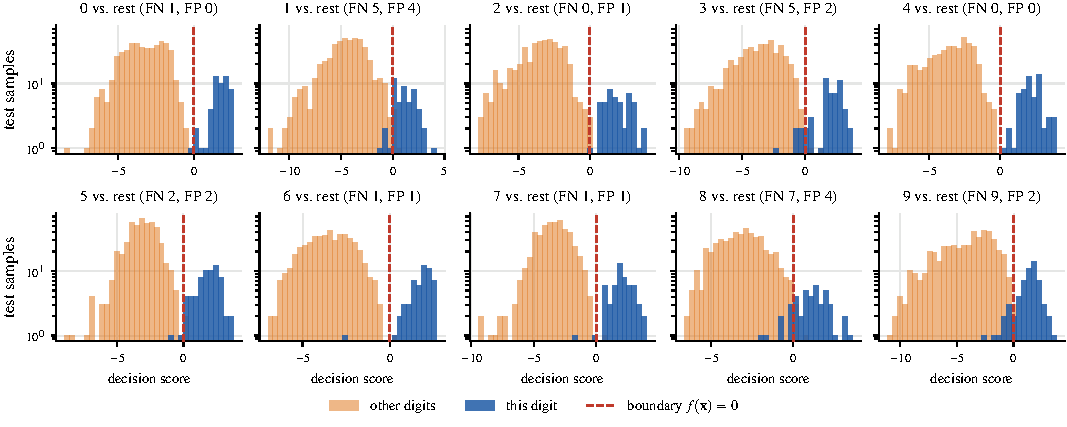
\includegraphics[width=\textwidth]{svm_scores.pdf}
\caption{SVM decision boundaries for the ten one-vs-rest classifiers. Each panel shows the test-set decision scores of the target digit (blue) and of all other digits (orange) on a log scale, with the boundary $f(\mathbf{x})=0$ in red. FN: images of the digit scored below 0; FP: other digits scored above 0.}
\label{fig:svm_scores}
\end{figure*}

To also see the boundaries in the input space, we projected the data onto its first two principal components and retrained the SVM in 2-D (Fig.~\ref{fig:svm_pca}). The boundaries are straight lines, as expected for a linear model. Two components keep only 22\% of the variance, so the 2-D accuracy drops to 40--45\%. Digits 0, 2, 4 and 6 still have clear regions, while the others overlap in the middle. A larger $\lambda$ shrinks the weights, so some small class regions disappear and the accuracy drops slightly.

\begin{figure*}[t]
\centering
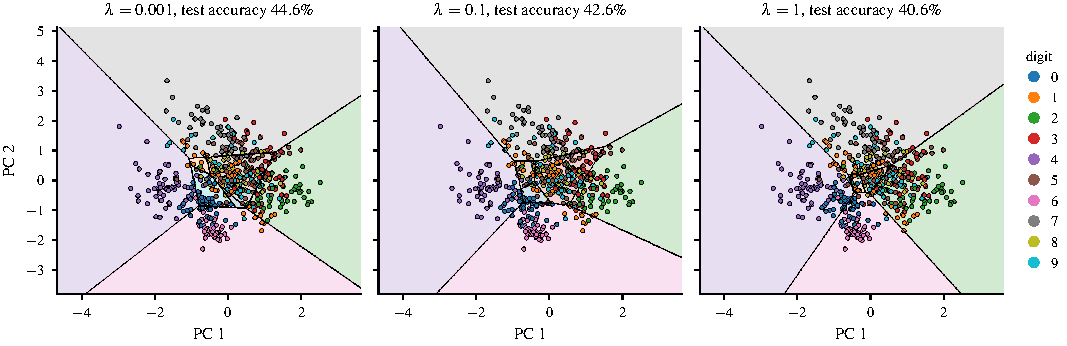
\includegraphics[width=\textwidth]{pca.pdf}
\caption{SVM decision regions in the first two principal components for $\lambda=0.001$, 0.1 and 1. Points are test samples coloured by their true digit.}
\label{fig:svm_pca}
\end{figure*}

\textit{MLP.} Fig.~\ref{fig:tuning}(c)--(d) shows that adding hidden units helps up to 256 units. A very small learning rate learns too slowly, and a very large one starts to hurt accuracy. The best setting was $H=256$ and $\eta=0.5$. Training accuracy reaches 100\% after about 100 epochs, but the CV accuracy keeps rising slowly up to 8000 epochs, so longer training did not cause overfitting. We therefore trained the final MLP for 8000 epochs, and it reached 98.0\% test accuracy.

\textit{Comparison.} The best random forest used 300 trees with no depth limit, $\sqrt{n}$ features per split and a minimum leaf size of 1. Table~\ref{tab:clf} compares the three classifiers. The MLP makes 11 errors on 540 test images, the random forest 15 and the SVM 18, and the ranking is the same under CV. The confusion matrices (Fig.~\ref{fig:conf}) show that most mistakes involve similar-looking digits such as 1, 3, 8 and 9. The SVM can only draw linear boundaries, whereas the MLP and the random forest can capture non-linear patterns, which explains their small advantage.

\begin{table}[t]
\centering
\small
\caption{Digits classification results on the test set}
\label{tab:clf}
\setlength{\tabcolsep}{4pt}
\begin{tabular}{lcccc}
\toprule
Model & CV acc. & Train acc. & Test acc. & Errors\\
\midrule
Multiclass SVM (ours) & 0.9547 & 0.9825 & 0.9667 & 18\\
MLP (ours) & \textbf{0.9801} & 1.0000 & \textbf{0.9796} & \textbf{11}\\
RandomForest (sklearn) & 0.9745 & 1.0000 & 0.9722 & 15\\
\bottomrule
\end{tabular}
\end{table}

\begin{figure*}[t]
\centering
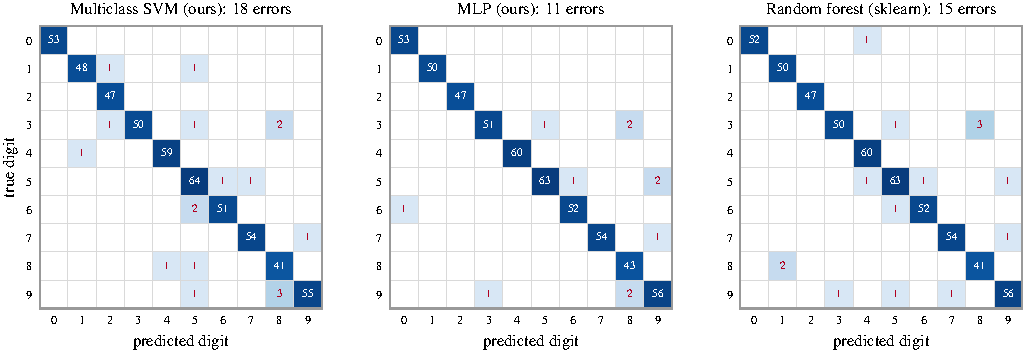
\includegraphics[width=\textwidth]{conf.pdf}
\caption{Test-set confusion matrices for the SVM, the MLP and the random forest. Diagonal cells are correct predictions; empty cells are zero.}
\label{fig:conf}
\end{figure*}

\subsection{Return prediction}
\textit{Tuning (2001--2010).} For Lasso, we tried windows of 5, 10 and 20 years and four values of the penalty $\alpha$. A 10-year window with $\alpha=10^{-4}$ was best (Sharpe ratio 1.51): five years seem too noisy, and twenty years include relationships that no longer hold. Larger values of $\alpha$ removed useful features. Since $10^{-4}$ is the smallest value in the grid, every feature kept a non-zero weight and Lasso behaved almost like least squares. The Lasso weights were very stable from year to year. For the random forest, we tried three depths and chose depth 8 (Sharpe ratio 2.68). The deeper version scored slightly higher, but it changed positions faster than once per day and was more likely to overfit. For the MLP, one hidden layer of 32 units worked best (Sharpe ratio 2.43). Both non-linear models beat Lasso, but they held positions for only about one day.

\textit{Smoothing.} Fig.~\ref{fig:smooth} shows the trade-off between the Sharpe ratio and the holding period. Smoothing makes positions last longer but lowers the Sharpe ratio, especially for the random forest and the MLP. Lasso is less affected. We chose $h=2$ as a compromise.

\begin{figure}[t]
\centering
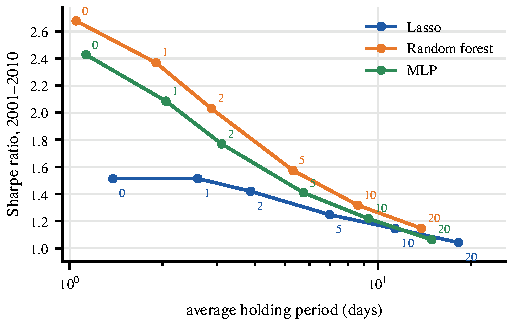
\includegraphics[width=\columnwidth]{smooth.pdf}
\caption{Validation Sharpe ratio against holding period for different smoothing half-lives $h$ (labels, in days).}
\label{fig:smooth}
\end{figure}

\begin{figure*}[t]
\centering
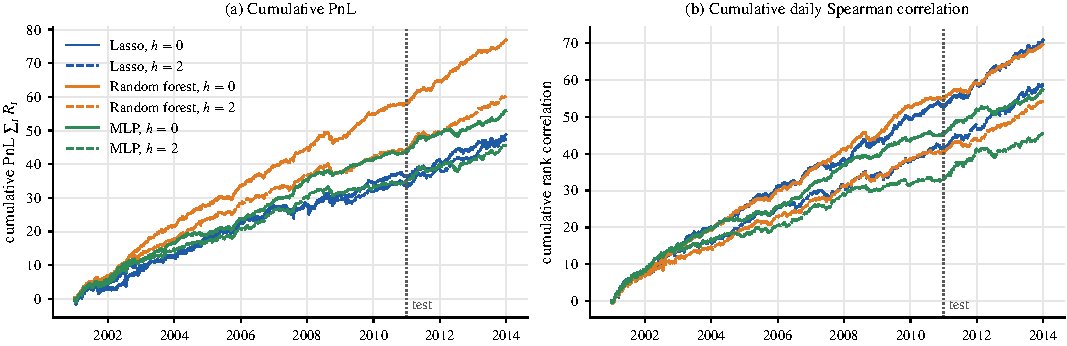
\includegraphics[width=\textwidth]{pnl.pdf}
\caption{Cumulative PnL (a) and cumulative daily rank correlation (b), 2001--2013. The dotted line marks the start of the test period. Solid lines: no smoothing; dashed lines: $h=2$.}
\label{fig:pnl}
\end{figure*}

\textit{Test results (2011--2013).} Table~\ref{tab:test} shows the metrics of~\eqref{eq:sharpe} and~\eqref{eq:hold} for each strategy. All six strategies had a positive Sharpe ratio on the test years and predicted at least 494 stocks every day. The unsmoothed random forest scored highest (4.03), but it held positions for less than a day. Smoothed Lasso offered the best balance, with a Sharpe ratio of 1.96 and a holding period of 4.3 days. The assignment suggests that a Sharpe ratio of 0.8--1 is already interesting at a 3--5 day holding period. With three years of test data, the standard error of the Sharpe ratio is about $1/\sqrt{3}\approx0.58$, so even the weakest result (1.71) is clearly above zero. The correlation with the market (0.17--0.42) is not zero. The portfolio is neutral in volatility-adjusted terms, but the low-volatility feature favours calm stocks, which receive larger dollar positions, so the dollar exposure is slightly net long.

\begin{table}[t]
\centering
\small
\caption{Test results, 2011--2013}
\label{tab:test}
\begin{tabular}{lcccc}
\toprule
Strategy & Sharpe & Rank corr. & Hold. (days) & Mkt corr.\\
\midrule
Lasso, $h=0$ & 1.90 & 0.023 & 1.31 & 0.32\\
Lasso, $h=2$ & 1.96 & 0.022 & \textbf{4.26} & 0.32\\
RF, $h=0$ & \textbf{4.03} & 0.020 & 0.90 & 0.35\\
RF, $h=2$ & 2.89 & 0.018 & 2.29 & 0.42\\
MLP, $h=0$ & 2.47 & 0.016 & 1.06 & \textbf{0.17}\\
MLP, $h=2$ & 1.71 & 0.016 & 2.94 & 0.19\\
\bottomrule
\end{tabular}
\end{table}

Fig.~\ref{fig:pnl} shows that the PnL and the cumulative rank correlation rise steadily over 2001--2013, with no long losing periods, and the test years look much like the validation years. Table~\ref{tab:sub} shows that 2006--2010 was the weakest sub-period for every model. Every model had a positive Sharpe ratio in each of the 13 years, with the weakest years during the 2007--2008 financial crisis.



\begin{table}[t]
\centering
\small
\caption{Sharpe ratio by sub-period (for $h=2$, smoothing runs continuously from 2001, so the 2011--13 values differ slightly from Table~\ref{tab:test})}
\label{tab:sub}
\begin{tabular}{lcccc}
\toprule
Strategy & 2001--05 & 2006--10 & 2011--13 & 2001--13\\
\midrule
Lasso, $h=0$ & 1.83 & 1.18 & 1.90 & 1.59\\
Lasso, $h=2$ & 1.83 & 0.98 & 1.98 & 1.54\\
RF, $h=0$ & 2.89 & 2.45 & 4.03 & 2.90\\
RF, $h=2$ & 2.44 & 1.57 & 2.90 & 2.20\\
MLP, $h=0$ & 2.31 & 2.66 & 2.47 & 2.43\\
MLP, $h=2$ & 1.88 & 1.67 & 1.77 & 1.77\\
\bottomrule
\end{tabular}
\end{table}

\textit{Sentiment.} We added two features from the Psychsignal data: net sentiment (bullish minus bearish) and activity (bullish plus bearish), each averaged over a week, with stocks that have no messages set to 0 (neutral). Because these data start in mid-2009, we retrained Lasso on up to three years of data, with and without them. Because of this shorter window, the baseline differs from Table~\ref{tab:test}. Sentiment raised the test Sharpe ratio from 1.78 to 1.92, or from 1.52 to 1.61 with smoothing. Given the limited coverage and the standard error of about 0.58, we do not consider this gain meaningful.

\section{Discussion and Conclusion}
On Diabetes, our Lasso and ElasticNet slightly beat least squares (test MSE 2797 and 2809, versus 2822). Their main benefit is simpler and more interpretable weights when features are correlated. Our ElasticNet never set weights exactly to zero. Using the proximal ElasticNet update from Lecture~8, $\vect{w}\leftarrow S_{\eta\lambda_1}(\vect{v})/(1+\eta\lambda_2)$, would fix this. On Digits, the MLP (98.0\%) beat the random forest (97.2\%) and the linear SVM (96.7\%). Some non-linearity helps, although the linear model already performs well.

For stock returns, simple reversal, momentum and volatility features gave positive and fairly steady Sharpe ratios out of sample. The random forest and the MLP scored highest but traded almost daily, while Lasso was more stable and worked best once smoothed. The main limitations are that we ignored trading costs, which would hurt the fast strategies most, and that our grids for the non-linear models were small. In future work, we would add trading costs, control turnover more directly, remove sector effects and test more features while guarding against false discoveries.

\section{Statement of Contributions}
Jack McDonald and William Charron-Boyle completed Tasks~1 and~2: the data analysis, the four from-scratch models and the comparison with scikit-learn. Radman Jamalshirpanjeh and Brandon Ku completed Task~3: the volatility adjustment, the features, the rolling training and evaluation, and the sentiment experiment. Each pair reviewed its own part of the notebook and wrote the corresponding sections of this report.

\textit{Use of large language models.} We used LLMs in a limited, supporting role. Before writing any Task~3 code, we asked LLMs to explain the task's expectations and equations, using the prompt: ``Explain Task 3 of this assignment step by step so I understand the expectations. For each equation, explain what it computes and why it is used.'' During coding, LLMs were also used to check the notebook against the assignment instructions and to revise a few notebook cells (the 2001--2013 Sharpe and PnL plots and some markdown summaries). For the report, they produced the initial IEEE template, formatted the tables and figures, and helped draft and edit the wording. All models, experiments and results come from our own notebook, and we checked every number in the report.

\begin{thebibliography}{99}
\bibitem{notes} M. Coates, \emph{ECSE 551: Machine Learning for Engineers, Lecture Notes} (Lectures 3, 4, 6, 7, 8 and 9), McGill University, Fall 2026.
\bibitem{numpy} NumPy Developers, ``NumPy documentation,'' [Online]. Available: \url{https://numpy.org/doc/stable/}
\bibitem{skDiab} scikit-learn Developers, ``load\_diabetes,'' scikit-learn documentation. [Online]. Available: \url{https://scikit-learn.org/stable/modules/generated/sklearn.datasets.load_diabetes.html}
\bibitem{skDig} scikit-learn Developers, ``load\_digits,'' scikit-learn documentation. [Online]. Available: \url{https://scikit-learn.org/stable/modules/generated/sklearn.datasets.load_digits.html}
\bibitem{skLinReg} scikit-learn Developers, ``LinearRegression,'' scikit-learn documentation. [Online]. Available: \url{https://scikit-learn.org/stable/modules/generated/sklearn.linear_model.LinearRegression.html}
\bibitem{skRF} scikit-learn Developers, ``Ensembles: Random forests,'' scikit-learn User Guide. [Online]. Available: \url{https://scikit-learn.org/stable/modules/ensemble.html}
\bibitem{skGS} scikit-learn Developers, ``GridSearchCV,'' scikit-learn documentation. [Online]. Available: \url{https://scikit-learn.org/stable/modules/generated/sklearn.model_selection.GridSearchCV.html}
\bibitem{skKFold} scikit-learn Developers, ``KFold,'' scikit-learn documentation. [Online]. Available: \url{https://scikit-learn.org/stable/modules/generated/sklearn.model_selection.KFold.html}
\bibitem{skPre} scikit-learn Developers, ``Preprocessing data,'' scikit-learn User Guide. [Online]. Available: \url{https://scikit-learn.org/stable/modules/preprocessing.html}
\bibitem{skLasso} scikit-learn Developers, ``Lasso,'' scikit-learn documentation. [Online]. Available: \url{https://scikit-learn.org/stable/modules/generated/sklearn.linear_model.Lasso.html}
\bibitem{skMLP} scikit-learn Developers, ``MLPRegressor,'' scikit-learn documentation. [Online]. Available: \url{https://scikit-learn.org/stable/modules/generated/sklearn.neural_network.MLPRegressor.html}
\end{thebibliography}

\end{document}
